\chapter{Controller Design}

This section outlines the basic architecture used for the inner loop flight controllers.
These flight controllers will be used to stabilize the GHV during flight, and track desired reference commands.
The modal analysis showed the decoupling of the velocity, longitudinal, and lateral modes, allowing each of these three subsystems to be considered independently.
This allows the control design of the GHV to be simplified, by having to design three lower order controllers, as opposed to a single higher order controller.
The velocity and longitudinal subsystems are both single input systems.
The throttle input $u_{\text{th}}$ controls only the velocity $V_{T}$, and the elevator input $u_{\text{elv}}$ controls the longitudinal states.
The lateral subsystem is multi input, with the aileron $u_{\text{ail}}$ and tail $u_{\text{rud}}$ as control inputs.
The resulting control block diagram is using the three decoupled subsystem controllers is shown in Figure (\ref{innercont_block_fig}).
The regulated outputs for each of the three subsystems is shown on the left of the figure, and the states used in the feedback loop of each of the control subsystems are shown as well.

\begin{figure}[h]
  \begin{center}
    \begin{tikzpicture}[scale=1.0, auto, node distance=2cm,>=latex']
      \matrix[ampersand replacement=\&, row sep=0.7cm, node distance=3.0cm] (regions) at (0,0){%
      \node[block, minimum width=3cm] (R1) {\shortstack{Velocity \\ Controller}}; \\
      \node[block, minimum width=3cm] (R2) {\shortstack{Longitudinal \\ Controller}};\\
      \node[block, minimum width=3cm] (R3) {\shortstack{Lateral \\ Controller}};\\
      };
      \matrix[ampersand replacement=\&, row sep=0.6cm, right of=R1, node distance=4.0cm] (R1out) {%
      \node [coordinate] (R1outx) {};\\
      \node [coordinate] (R1outP) {};\\
      };
      \matrix[ampersand replacement=\&, row sep=0.6cm, right of=R2, node distance=4.0cm] (R2out) {%
      \node [coordinate] (R2outx) {};\\
      \node [coordinate] (R2outP) {};\\
      };
      \matrix[ampersand replacement=\&, row sep=0.6cm, right of=R3, node distance=4.0cm] (R3out) {%
      \node [coordinate] (R3outx) {};\\
      \node [coordinate] (R3outP) {};\\
      };
      \node [coordinate, left of=R1, node distance=3.5cm] (input1) {};
      \node [coordinate, left of=R2, node distance=3.5cm] (input2) {};
      \matrix[ampersand replacement=\&, row sep=0.6cm, left of=R3, node distance=3.5cm] (R3in) {%
      \node [coordinate] (R3inx) {};\\
      \node [coordinate] (R3inP) {};\\
      };
      \node [coordinate, right of=R3inx, node distance=2.0cm] (R3inx2) {};
      \node [coordinate, right of=R3inP, node distance=2.0cm] (R3inP2) {};
      \node [block, right of=R2,node distance=6.0cm, minimum width=4cm, minimum height=6cm] (Q) {\shortstack{GHV \\ Dynamics}};
      %Region 1 outputs
      \draw [->] (R1.east) + (0cm,0.3cm) -- node [pos=0.5]{$u_{\text{th}}$} (R1outx);
      \draw [<-] (R1.east) + (0cm,-0.3cm) -- node [pos=0.5]{$V_{T}$} (R1outP);
      %Region 2 outputs
      \draw [->] (R2.east) + (0cm,0.3cm) -- node [pos=0.5]{$u_{\text{elv}}$} (R2outx);
      \draw [<-] (R2.east) + (0cm,-0.3cm) -- node [pos=0.5]{$\alpha$, $q$} (R2outP);
      %Region 3 outputs
      \draw [->] (R3.east) + (0cm,0.3cm) -- node [pos=0.5]{$u_{\text{ail}}$, $u_{\text{rud}}$} (R3outx);
      \draw [<-] (R3.east) + (0cm,-0.3cm) -- node [pos=0.5]{$\beta$, $p$, $r$, $\phi$} (R3outP);
      %INPUTS
      \draw [->] (input1) -- node [near start]{$V_{T,\text{cmd}}$} (R1);
      \draw [->] (input2) -- node [near start]{$\alpha_{\text{cmd}}$} (R2);
      % Region 3 outputs
      \draw [->] (R3inx) -- node [near start]{$\phi_{\text{cmd}}$} (R3inx2);
      \draw [->] (R3inP) -- node [near start]{$\beta_{\text{cmd}}$} (R3inP2);
    \end{tikzpicture}
    \caption{Inner loop flight control block diagram\label{innercont_block_fig}}
  \end{center}
\end{figure}

In this chapter, the details regarding control strategy that will be used on each of the three control blocks will be presented, as well as some details concerning the individual subsystems themselves.
This includes a baseline control design and analysis, as well as adaptive augmentation for the longitudinal and lateral subsystems.
It is assumed that the state is available for measurement.

\section{Baseline Control Architecture}
The nominal, linear equations of motion describing each of the three subsystems are described by Equation (\ref{eqn:plantxp}) with the addition of the regulated output $z$ as
\begin{equation}
  \label{eqn:xdotp}
  \begin{split}
    \dot{x}_{p}&=A_{p}x_{p}+B_{p}u \\
    z&=C_{zp}x_{p} \\
  \end{split}
\end{equation}
where $x_{p}\in\mathbb{R}^{n_{p}}$, $u\in\mathbb{R}^{m}$, $A_{p}\in\mathbb{R}^{n_{p}\times n_{p}}$, $B_{p}\in\mathbb{R}^{n_{p}\times m}$,$C_{pz}\in\mathbb{R}^{n_{e}\times n_{p}}$, and $z\in\mathbb{R}^{n_{e}}$.
Note again that the dimensions of each of these quantities may differ for each of the three control subsystems.
Each linear plant subsystem is controlled using an LQR-PI full state feedback controller.
The LQR-PI control architecture is most easily represented by augmenting the plant state with an additional integral error state as follows.
Define the integral error state as the difference between a reference command and corresponding regulated output given by
\begin{equation}
  \label{eqn:integralerror}
  \dot{x}_{e}=z_{\text{cmd}}-z
\end{equation}
In this work the regulated outputs happen to all be components of the state vector, but in general this does not have to be the case, and is the motivation for using the general description of the regulated output.
Using the error description in (\ref{eqn:integralerror}), the state vector $x_{p}$ is augmented to include this error by including $x_{e}$ as a state variable
\begin{equation}
  \label{lqrpi_linear_ss_eqn}
  \begin{bmatrix}
    \dot{x}_{p} \\
    \dot{x}_{e}
  \end{bmatrix}
  =
  \begin{bmatrix}
    A_{p} & 0 \\
    -C_{pz} & 0
  \end{bmatrix}
  \begin{bmatrix}
    x_{p} \\
    x_{e}
  \end{bmatrix}
  +
  \begin{bmatrix}
    B_{p} \\
    0
  \end{bmatrix}u
  +
  \begin{bmatrix}
    0 \\
    I
  \end{bmatrix}z_{\text{cmd}}
\end{equation}
Writing the linear state-space representation in Equation~\ref{lqrpi_linear_ss_eqn} more compactly using $x=\bigr[\begin{array}{cc} x_{p}^{\top} & x_{e}^{\top} \end{array}\bigr]^{\top}$ as
\begin{equation}
  \label{lqrpiss}
  \dot{x}=Ax+Bu+B_{\text{ref}}z_{\text{cmd}}
\end{equation}
where $x\in\mathbb{R}^{n}$, $z_{\text{cmd}}\in\mathbb{R}^{n_{e}}$, $A\in\mathbb{R}^{n\times n}$, $B\in\mathbb{R}^{n\times m}$, $B_{\text{ref}}\in\mathbb{R}^{n\times n_{e}}$ and where
\begin{equation}
  A=
  \begin{bmatrix}
    A_{p} & 0 \\
    -C_{pz} & 0
  \end{bmatrix} \quad
  B=
  \begin{bmatrix}
    B_{p} \\
    0
  \end{bmatrix}
  \quad
  B_{\text{ref}}=
  \begin{bmatrix}
    0 \\
    I
  \end{bmatrix}
\end{equation}
The following baseline control law is used
\begin{equation}
  \label{lqrpilaw}
  u_{\text{bl}}=K_{\text{lqr}}^{\top}x
\end{equation}
Substituting the control law (\ref{lqrpilaw}) into (\ref{lqrpiss})
\begin{equation}
  \label{eqn:nomaugmentedss}
  \dot{x}=\left(A+BK_{\text{lqr}}^{\top}\right)x+B_{\text{ref}}z_{\text{cmd}}
\end{equation}
The gain $K_{\text{lqr}}\in\mathbb{R}^{n\times m}$ is selected by minimizing the cost function (\ref{eqn:jcostfunction}), and ensures the closed loop matrix $\left(A+BK_{\text{lqr}}^{\top}\right)$ is Hurwitz.
The matrices $Q_{\text{lqr}}=Q_{\text{lqr}}^{\top}>0$ and $R_{\text{lqr}}=R_{\text{lqr}}^{\top}>0$ are weights which impact the calculation of the feedback gain.
The selection of these matrices and the resulting effect on control performance is discussed in following sections.
\begin{equation}
  \label{eqn:jcostfunction}
  J=\int_{0}^{\infty}\bigr(x(t)^{\top}Q_{\text{lqr}}x(t)+u(t)^{\top}R_{\text{lqr}}u(t)\bigr)dt
\end{equation}
The optimal feedback gain $K_{\text{lqr}}$ for the control law $u=K_{\text{lqr}}^{\top}x$ is then found by solving the following algebraic Riccati equation.
\begin{equation}
  0=A^{\top}P+PA+Q_{\text{lqr}}-PBR_{\text{lqr}}^{-1}B^{\top}P
\end{equation}
where $K_{\text{lqr}}=-(R_{\text{lqr}}^{-1}B^{\top}P)^{\top}$.

\subsubsection*{The Three Control Subsystems}

The three subsystems that the plant was separated into allowed multiple lower order controllers.
Each of the subsystems of the plant for which a controller will be designed is outlined here.

\paragraph{Velocity}
From the sensitivity analysis, the total velocity is decoupled from the rest of the states, allowing a separate controller to be designed to regulate and control only velocity.
The perturbation state and input used in the velocity controller is
\begin{equation}
  \begin{split}
    x_{p,\text{vtot}}&=
    \bigr[
    \begin{array}{c}
      V_{T}
    \end{array}\bigr] \\
    u_{\text{vtot}}&=
    \bigr[
    \begin{array}{c}
      \delta_{\text{th}}
    \end{array}\bigr]
  \end{split}
\end{equation}
For the velocity subsystem $n_{p}=1$ and $m=1$.
Integral action is applied for tracking velocity reference commands.
That is $n_{e}=1$ and $C_{pz}=\bigr[\begin{array}{c}1\end{array}\bigr]$.

\paragraph{Longitudinal}
The longitudinal system as shown through the modal analysis is decoupled from the other subsystems.
In addition to this decoupling, the longitudinal subsystem can be simplified even further by omitting the pitch angle and altitude states.
This is because they are much slower than the pitch rate and angle of attack.
This subsystem has perturbation state vector
\begin{equation}
  \label{long_statevector_eqn}
  \begin{split}
    x_{p,\text{long}}&=
    \bigr[
    \begin{array}{cc}
      \alpha & q
    \end{array}\bigr]^{\top} \\
    u_{\text{long}}&=
    \bigr[
    \begin{array}{c}
      \delta_{\text{elv}}
    \end{array}\bigr]
  \end{split}
\end{equation}
and $n_{p}=2$ and $m=1$.
Integral action is applied for tracking angle of attack reference commands.
That is $n_{e}=1$ and $C_{pz}=\bigr[\begin{array}{cc}1 & 0 \end{array}\bigr]$.

\paragraph{Lateral-Directional States}
The lateral-directional has perturbation state vector
\begin{equation}
  \label{lat_statevector_eqn}
  \begin{split}
    x_{p,\text{latr}}&=
    \bigr[
    \begin{array}{cccc}
      \beta & p & r & \phi
    \end{array}\bigr]^{\top} \\
    u_{\text{latr}}&=
    \bigr[
    \begin{array}{cc}
      \delta_{\text{ail}} & \delta_{\text{rud}}
    \end{array}\bigr]^{\top}
  \end{split}
\end{equation}
and $n_{p}=4$ and $m=2$.
Because there are two independent control inputs, integral action is applied for tracking both angle of sideslip, and roll angle reference commands.
That is $n_{e}=2$ and
\begin{equation}
  C_{pz}=
  \left[
  \begin{array}{cccc}
    1 & 0 & 0 & 0 \\
    0 & 0 & 0 & 1
  \end{array}\right]
\end{equation}

\section{Frequency-Domain Analysis}

Each of the three control subsystems presented above can be represented using the standard servo, or tracking configuration block diagram in Figure~\ref{fig.lqrpiblock}, where $d_{\text{in}}$ is an input load disturbance, $d_{\text{out}}$ is an output load disturbance or sensor bias, and $n$ is sensor noise.
This representation facilitates the following frequency domain analysis of each of the plant and control subsystems, and is different from the conventional representation only by the addition of the reference signal $z_{\text{cmd}}$.
Additionally, with the LQR-PI controller $r=0$.
The frequency domain analysis is done by breaking the loop at various break points, namely at the input to and output from the plant $G(s)$, with the reference command $z_{\text{cmd}}$ set to zero.
At each of these break points the loop transfer function is found and a sinusoidal signal applied at break point input.
The magnitude and phase of the signal when measured at the break point output provides valuable information about the robustness of the control system\ \cite{book.astrommurray.2009}.

\begin{figure}[H]
  \begin{center}
    \begin{tikzpicture}[auto, scale=1.0, every node/.style={transform shape}, node distance=1.0cm, >=latex']
      \node[squareblock, minimum height=2cm, minimum width=2cm, label=above:{Controller}] (block1){$K(s)$};
      \node[left=of block1.150, node distance=5.0cm] (j1) {};
      \node[left of=j1, node distance=1.9cm] (input1) {};
      \node[whitesum,left=of block1.200, node distance=1.5cm] (sum1) {};
      \node[input, left of=sum1, node distance=1.5cm](input2){};
      \node[whitesum, right of=block1, node distance=2.5cm] (sum2) {};
      \node[input, above of=sum2,node distance=1.5cm](input3){};
      \node[squareblock, minimum height=2cm, minimum width=2cm, right of=sum2, label=above:{Plant},node distance=2.5cm] (block2) {$G(s)$};
      \node[whitesum, right of=block2,node distance=2.5cm] (sum3) {};
      \node[input, above of=sum3,node distance=1.5cm](input4){};
      \node[output, right of=sum3,node distance=2.5cm] (output1) {};
      \draw[->](sum3) --  node[name=yi,pos=0.4]{$y_{i}$}(output1);
      \node[whitesum, below of=yi,node distance=2.5cm] (sum4) {};
      \node[input, right of=sum4,node distance=1.5cm](input5){};
      \draw[->](input1) -- node[near start]{$z_{\text{cmd}}$} (block1.150);
      \draw[->](input2) -- node[near start]{$r$} node[pos=0.9] {$+$} (sum1);
      \draw[->](sum1) -- node{$e$} (block1.200);
      \draw[->](block1) -- node{$u_{o}$} node[pos=0.9]{$+$} (sum2);
      \draw[->](input3) -- node[near start]{$d_{\text{in}}$} node[pos=0.9] {$+$} (sum2);
      \draw[->](sum2) -- node{$u_{i}$} (block2);
      \draw[->](block2) -- node{$y_{o}$} node[pos=0.95] {$+$} (sum3);
      \draw[->](input4) -- node[near start]{$d_{\text{out}}$} node[pos=0.9] {$+$} (sum3);
      \draw[->](yi) -- node[pos=0.9] {$+$} (sum4);
      \draw[->](input5) -- node[near start]{$n$} node[pos=0.9] {$-$} (sum4);
      \draw[->](sum4) -| node{$w$} node[pos=0.95] {$-$} (sum1);
    \end{tikzpicture}
    \caption{General MIMO feedback control block diagram\label{fig.lqrpiblock}}
  \end{center}
\end{figure}

This frequency domain analysis guides the selection of the weighting matrices in (\ref{eqn:jcostfunction}) which ultimately dictate the corresponding feedback gain.
By completing a frequency domain analysis, the weighting matrices are adjusted until satisfactory level of robustness is achieved.

\subsection{The Different Loop Transfer Functions}

The following give various transfer functions for a plant and controller system represented by Figure~\ref{fig.lqrpiblock}.
The following are titled as transfer functions, but they could actually be transfer matrices.
In the case of SISO systems, multiplication is commutative, but care was taken in the following expressions to consider the MIMO case and preserve pre- and post- multiplication when making algebraic manipulations.
It is also worth noting that many of the other transfer functions between the inputs $r$, $d_{\text{in}}$, $d_{\text{out}}$, and $n$ and the five outputs are described by the transfer functions below, but the transfer functions will be described as relationships between the input and output which is of greatest interest in analyzing the control system.
In the following section $I$ is used to denote the identity matrix, where the size is obvious.

\subsubsection{Input}

\paragraph{Loop Gain Transfer Function}
Breaking the loop at the plant input, the transfer function from $u_{i}$ to $u_{o}$ is given by
\begin{equation}
  L_{u}(s)=K(s)G(s)
\end{equation}

\paragraph{Return Difference Transfer Function}
Differencing the input $u_{i}$ and output $u_{o}$ gives the return difference transfer function
\begin{equation}
  I+L_{u}(s)
\end{equation}

\paragraph{Sensitivity Transfer Function}
The input sensitivity transfer function is from $d_{\text{in}}$ to $u_{i}$ and is given by
\begin{equation}
  S_{u}(s)=\bigr(I+L_{u}(s)\bigr)^{-1}
\end{equation}

\paragraph{Complementary Sensitivity Transfer Function}
Unlike the $T_{y}(s)$, the input complementary sensitivity transfer function does not represent an relationship between any of the system inputs and outputs.
This transfer function is given by using the identity $S_{u}(s)+T_{u}(s)=I$, hence the name complementary sensitivity transfer function, but otherwise there is little intuition regarding what this transfer function represents, and it won't be used in the frequency domain analysis.
\begin{equation}
  T_{u}(s)=L_{u}(s)\bigr(I+L_{u}(s)\bigr)^{-1}
\end{equation}
Note also that $L(I+L)^{-1}=(I+L)^{-1}L$ which can be shown by pre- and post- multiplying both sides by $(I+L)$.

\subsubsection{Output}
\paragraph{Loop Gain Transfer Function}
Evaluate the transfer function from break point input $y_{i}$ to break point output $y_{o}$ while all other signals are zero.
\begin{equation}
  L_{y}(s)=G(s)K(s)
\end{equation}

\paragraph{Return Difference Transfer Function}
Differencing the input $y_{i}$ and output $y_{o}$ gives
\begin{equation}
  I+L_{y}(s)
\end{equation}

\paragraph{Sensitivity Transfer Function}
The output sensitivity is from $d_{\text{out}}$ to $y_{i}$ with all other signals are zero.
\begin{equation}
  S_{y}(s)=\bigr(I+L_{y}(s)\bigr)^{-1}
\end{equation}

\paragraph{Complementary Sensitivity Transfer Function}
Unlike $T_{u}(s)$, this transfer function represents the relationship between the noise $n$ and the output $y_{o}$.
This transfer function also satisfies the identity $S_{y}(s)+T_{y}(s)=I$, hence the name complementary sensitivity transfer function.
\begin{equation}
  T_{y}(s)=L_{y}(s)\bigr(I+L_{y}(s)\bigr)^{-1}
\end{equation}

\subsubsection*{Representation of LQR-PI Controller}

In order to evaluate the loop transfer functions, the LQR-PI controller must be represented as a dynamic compensator, that is, a transfer matrix, as opposed to expressing it as an augmentation to the plant state space description.
Here the LQR-PI controller for the longitudinal subsystem is shown, and the process of expressing the other subsystem controllers this way is the same.
Because the longitudinal subsystem has two states and one input, the controller should be described by a system with three inputs (the reference command, and feedback from each of the two states) and one output.
The input to the controller is $\bigr[\begin{array}{ccc} \alpha_{\text{cmd}} & -\alpha & -q \end{array}\bigr]^{\top}$ and the output is $u$, in this case the commanded elevator deflection angle.
\begin{align}
  \dot{x}_{e}&=
  \begin{bmatrix}
    1 & 1 & 0
  \end{bmatrix}
  \begin{bmatrix}
    \alpha_{\text{cmd}} \\
    -\alpha \\
    -q
  \end{bmatrix} \\
  u&=
  \begin{bmatrix}
    k_{e}
  \end{bmatrix}
  \begin{bmatrix}
    x_{e}
  \end{bmatrix}+
  \begin{bmatrix}
    0 & -k_{\alpha} & -k_{q}
  \end{bmatrix}
  \begin{bmatrix}
    \alpha_{\text{cmd}} \\
    -\alpha \\
    -q
  \end{bmatrix}
\end{align}
The matrices corresponding this state space representation of the controller are the following
\begin{equation}
  A_{c}=0 \quad B_{c}=
  \begin{bmatrix}
    1 & 1 & 0
  \end{bmatrix}
  \quad C_{c}=
  \begin{bmatrix}
    k_{e}
  \end{bmatrix}
  \quad D_{c}=
  \begin{bmatrix}
    0 & -k_{\alpha} & -k_{q}
  \end{bmatrix}
\end{equation}
This state space representation was then converted to a transfer matrix representation for frequency domain analysis.
This transfer matrix was $1\times3$: from the controller input $r$, $-\alpha$, and $-q$ to the output $u_{\text{elv}}$.

\subsubsection*{Multivariable Frequency-Domain Analysis}

The controllers designed in the preceding section can be applied to the nonlinear model and simulated.
The feedback gains may be adjusted, and their performance evaluated using the simulation time response.
Stability can be checked by looking at the location of the closed-loop poles in the complex plane.
Even though the closed-loop system may be stable and respond very well for the nominal case, a lack of robustness could mean slight change in the plant parameters could cause the system to perform very poorly, and even become unstable.

The controller must be designed so the system performs well not only in the nominal case, but also when subject to disturbances such as wind gusts and sensor noise, and uncertainties in the plant parameters.
For SISO classical controllers, frequency domain tools such as the Bode plot are used.
The Bode for a single transfer function is not so easily extended to MIMO systems which is described by transfer function matrices.
Because of this, the singular values of the transfer matrices must be used.

In classical design the loop transfer function needed to be large at low frequency for good command following and disturbance rejection, but small at high frequency for noise attenuation.
When extending to transfer function matrices, a measure of the ``smallness'' of the matrix is needed: the singular values.
The singular value decomposition of a matrix $M$ is given by the factorization
\begin{equation}
  M=U\Sigma V^{*}
\end{equation}
where $(\cdot)^{*}$ denotes the Hermitian, or conjugate transpose, and $U$ and $V^{*}$ are real or complex unitary matrices, i.e. $U^{*}U=UU^{*}=I$, and $\Sigma$ is diagonal matrix with nonnegative real numbers on the diagonal.
The diagonal entries of $\Sigma$ are the singular values of $M$.
Taking the Hermitian transpose of $M$ gives $M^{*}=(U\Sigma V^{*})^{*}=V\Sigma^{*}U^{*}$.
Both pre- and post- multiplying $M$ with its Hermitian transpose:
\begin{equation}
  \begin{split}
    MM^{*}&=U\Sigma V^{*}V\Sigma^{*}U^{*}=U\Sigma \Sigma^{*}U^{*} \\
    M^{*}M&=V\Sigma^{*}U^{*}U\Sigma V^{*}=V\Sigma^{*}\Sigma V^{*}
  \end{split}
\end{equation}
Since $\Sigma$ is diagonal, this can be rearranged into the following eigenvalue problems, allowing the singular values to be found as the non-zero eigenvalues of $M^{*}M$ or $MM^{*}$.
\begin{equation}
  \begin{split}
    (MM^{*})U&=U(\Sigma \Sigma^{*}) \\
    (M^{*}M)V&=V(\Sigma^{*}\Sigma)
  \end{split}
\end{equation}
When the matrix $M$ is a transfer matrix $H(j\omega)$, the magnitude at a any frequency $\omega$ will depend on the direction of the input.
Different singular values will be excited depending on the input.
However, for any input the magnitude of $H(j\omega)$ is bounded above by its maximum singular value $\overline{\sigma}(H(j\omega))$ and below by its minimum singular value $\underline{\sigma}(H(j\omega))$.
To generate the singular value plot for the linear system $\dot{x}=Ax+Bu$ with output given by $y=Cx$, the transfer matrix $H$ must first be calculated:
\begin{equation}
  H(s)=C(sI-A)^{-1}B
\end{equation}
The singular values for each transfer matrix $H$ above can then be plotted versus frequency.
The following equations to determine the gain and phase margin for a MIMO system are found in Reference\ \cite{lavretskywise.book.2013} and presented here for completeness.
First define
\begin{equation}
  \alpha_{\sigma}=\min_{\omega}\underline{\sigma}\bigr(I+L_{u}(s)\bigr)
\end{equation}
\begin{equation}
  \beta_{\sigma}=\min_{\omega}\underline{\sigma}\bigr(I+L_{u}(s)^{-1}\bigr)
\end{equation}
Calculate the phase margin and gain margin from the return difference matrix as
\begin{equation}
  GM_{I+L}=\left[\frac{1}{1+\alpha_{\sigma}},\frac{1}{1-\alpha_{\sigma}}\right]\quad
  PM_{I+L}=\pm2\sin^{-1}\biggr(\frac{\alpha_{\sigma}}{2}\biggr)
\end{equation}
and from the stability robustness matrix as
\begin{equation}
  GM_{I+L^{-1}}=\left[1-\beta_{\sigma},1+\beta_{\sigma}\right]\quad
  PM_{I+L^{-1}}=\pm2\sin^{-1}\biggr(\frac{\beta_{\sigma}}{2}\biggr)
\end{equation}
Taking the union of these two gain and phase margin expressions yield the following multivariable margins.
\begin{equation}
  GM=GM_{I+L}\cup GM_{I+L^{-1}}\quad
  PM=PM_{I+L}\cup PM_{I+L^{-1}}
\end{equation}
These margins are more conservative than classical stability margins calculated for SISO systems.

\subsection{Closing Inner Flight Control Loops}

In this section the selection of the LQR weighting matrices and their impact on the frequency domain properties of the loop transfer functions is discussed.
The weighting matrices for each of the three baseline controllers are given, as well as the baseline feedback control gains that resulted.
Note that the units for the angle measurements used in feedback are radians, while the control surface deflections are in degrees, making many of the gains appear 57.3 times larger than what might be expected.
Note again that the frequency domain plots shown here are for the nominal flight condition.

\subsubsection*{Velocity Controller}

The design of the LQR-PI velocity controller followed the procedure as outlined above.
The values of the components of the LQR weighting matrices are given in Table~\ref{vtot_weights_tab}.
The velocity subsystem is open-loop stable, so the controller only had to provide the capability for reference command tracking.
Additionally, the throttle on aircraft, and hypersonic vehicles in particular, is adjust very slowly.
Because of this, the gains were kept relatively small, keeping the crossover frequency low, and the margins very conservative.

\begin{figure}[H]
  \begin{center}
    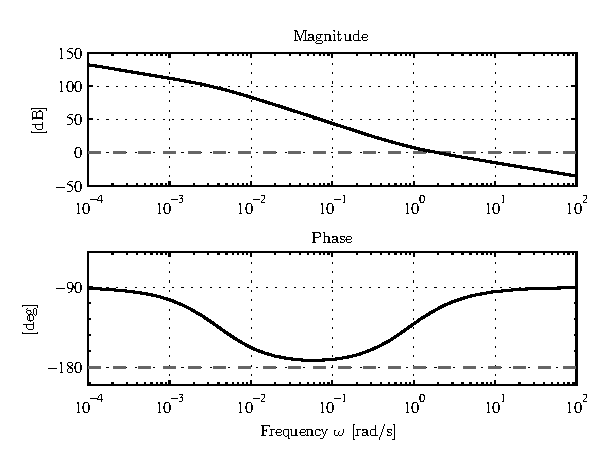
\includegraphics[width=4.0in]{\figurepath/results_vtotbode_v1.eps}
     \caption{Velocity loop transfer function Bode plot}
  \end{center}
\end{figure}

\begin{figure}[H]
  \begin{center}
    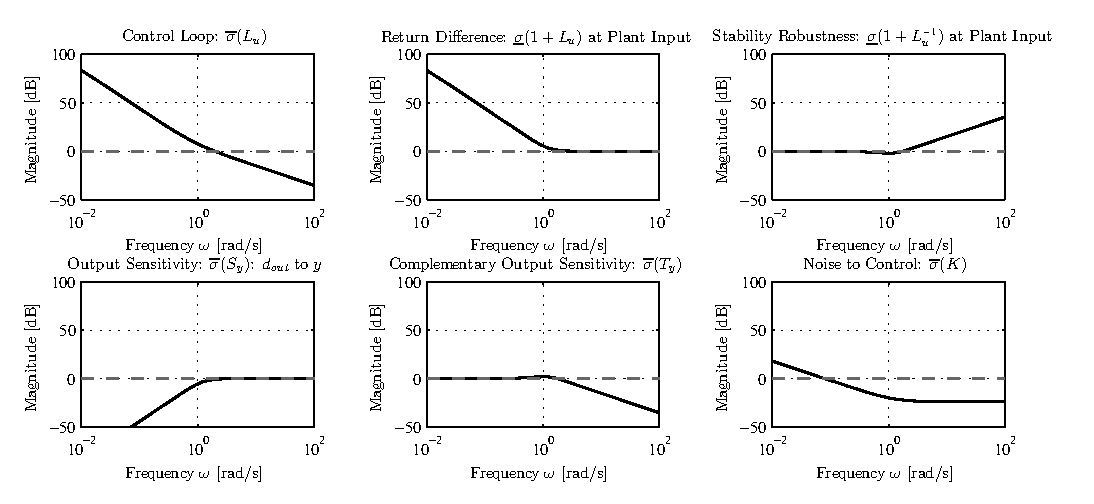
\includegraphics[width=6.5in]{\figurepath/results_vtotsigma_v1.eps}
     \caption{Velocity loop transfer function singular values}
  \end{center}
\end{figure}

\begin{table}[h]
  \centering
  \caption{Velocity controller LQR weights}
  \small
  \begin{tabular}{ccc}
    \toprule
    & Weight & Value \\
    \midrule
    \multirow{2}{*}{$Q_{\text{lqr}}$} & $V_{T}$ & 0 \\
    & $x_{e}$ & 1 \\
    \midrule
    $R_{\text{lqr}}$ & $u_{\text{th}}$ & 0.03 \\
    \bottomrule
  \end{tabular}\label{vtot_weights_tab}
\end{table}

\begin{equation*}
  {K_{\text{vtot}}}=
  \left[
  \begin{array}{cc}
    0.21 & -0.58
  \end{array}\right]^{\top}
\end{equation*}

\begin{equation*}
  GM=\text{Inf}
  \hspace{0.5in}
  PM=65.6\text{~deg}
\end{equation*}

\subsubsection*{Longitudinal Controller}

Unlike the velocity controller, the longitudinal dynamics of the GHV are highly unstable.
Because of this, the longitudinal control subsystem had to stabilize the plant in addition to providing reference command tracking.

\begin{figure}[H]
  \begin{center}
    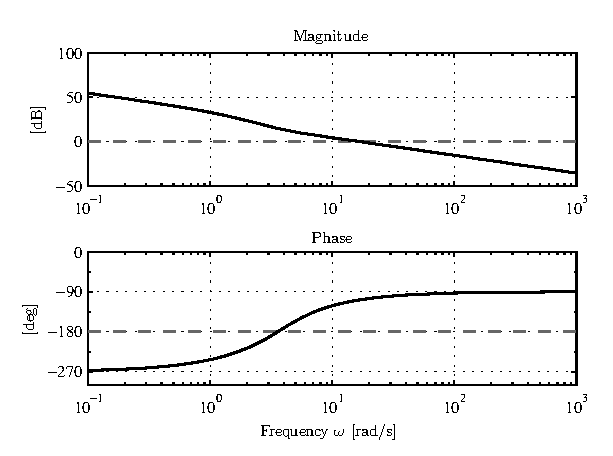
\includegraphics[width=4.0in]{\figurepath/results_longbode_v1.eps}
     \caption{Longitudinal loop transfer function Bode plot\label{fig:longbode}}
  \end{center}
\end{figure}

\begin{figure}[H]
  \begin{center}
    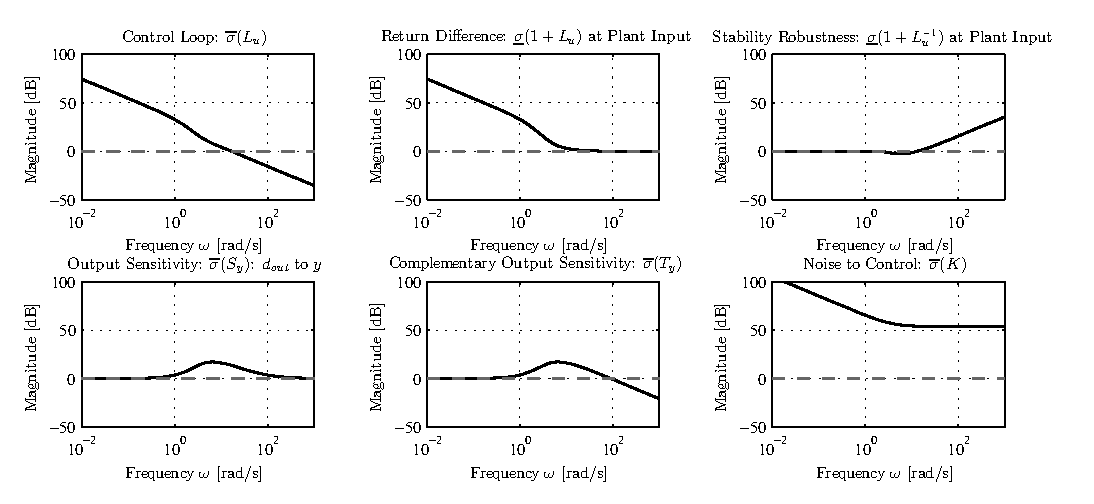
\includegraphics[width=6.5in]{\figurepath/results_longsigma_v1.eps}
     \caption{Longitudinal loop transfer function singular values\label{fig:longsigma}}
  \end{center}
\end{figure}

Also unlike the velocity subsystem the longitudinal control system should not be slow, although there is an upper limit on the crossover frequency based on the vehicle and actuator dynamics.
The Bode and singular value plots in Figure~\ref{fig:longbode} and Figure~\ref{fig:longsigma}, respectively, give a graphical representation of the frequency domain properties for this subsystem.

For this subsystem, tolerating a small crossover frequency in allowed a greater level of robustness to be achieved, at the expense of sacrificing the speed of the response.
While slow response characteristics might be acceptable for a large transport aircraft, the GHV must be able to quickly respond to commands in order to execute aggressive maneuvers.
Making the crossover frequency increasingly large eventually has diminishing returns, as due to the dynamics of the vehicle and the actuators, there is a limit on how quickly the vehicle can respond to commands.
Additionally, increasing the crossover frequency deteriorates the margins.
For this reason a crossover frequency of approximately 2 Hz was selected.

\begin{table}[H]
  \centering
  \caption{Longitudinal controller LQR weights}
  \small
  \begin{tabular}{ccc}
    \toprule
    & Weight & Value \\
    \midrule
    \multirow{3}{*}{$Q_{\text{lqr}}$} & $\alpha$ & 0 \\
    & $q$ & 0 \\
    & $x_{e}$ & 170 \\
    \midrule
    $R_{\text{lqr}}$ & $u_{\text{elv}}$ & 0.0001 \\
    \bottomrule
  \end{tabular}\label{long_weights_tab}
\end{table}

\begin{equation*}
  {K_{\text{long}}}=
  \left[
  \begin{array}{ccc}
    -434 & -67.8 & 1304
  \end{array}\right]^{\top}
\end{equation*}

\begin{equation*}
  GM=-14.8\text{~dB}
  \hspace{0.5in}
  PM=71.3\text{~deg}
\end{equation*}

\subsubsection*{Lateral-directional Controller}

The challenges associated with the design of the lateral controller were similar to that of the longitudinal controller in terms of an open loop unstable plant, and requirement for sufficiently large crossover.
The primary difference in the design of the lateral controller was that is multi-output.
This meant Bode plots could not be used, and the singular value plots had to be used.

\begin{figure}[h]
  \begin{center}
    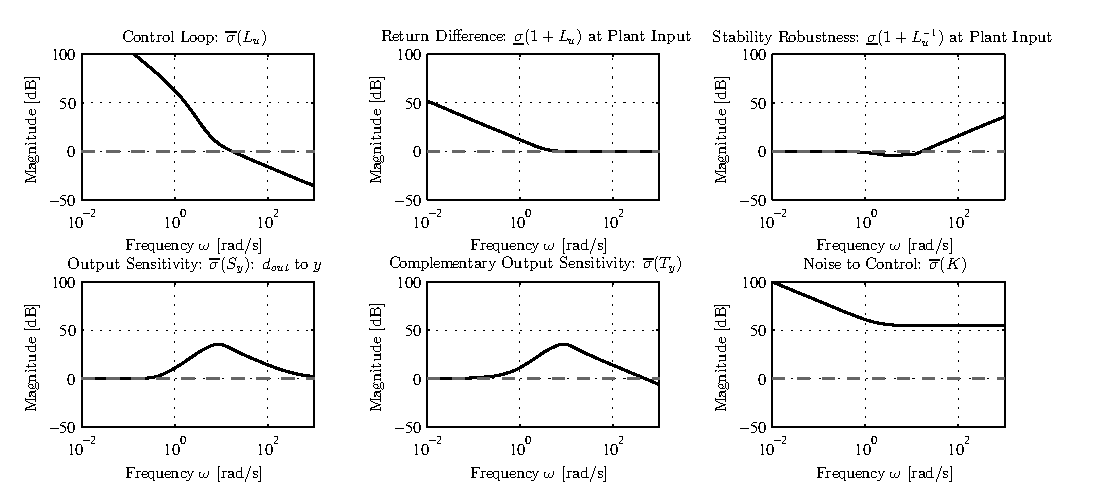
\includegraphics[width=6.5in]{\figurepath/results_latrsigma_v1.eps}
    \caption{Lateral loop transfer matrix singular values\label{fig:latrsigma}}
  \end{center}
\end{figure}

\begin{table}[h]
  \centering
  \caption{Lateral controller LQR weights}
  \small
  \begin{tabular}{ccc}
    \toprule
    & Weight & Value \\
    \midrule
    \multirow{6}{*}{$Q_{\text{lqr}}$} & $\beta$ & 0 \\
    & $p$ & 0 \\
    & $r$ & 0 \\
    & $\phi$ & 10 \\
    & $x_{e,\beta}$ & 10000 \\
    & $x_{e,p}$ & 100 \\
    \midrule
    \multirow{2}{*}{$R_{\text{lqr}}$} & $u_{\text{ail}}$ & 0.02 \\
    & $u_{\text{rud}}$ & 0.02 \\
    \bottomrule
  \end{tabular}\label{latr_weights_tab}
\end{table}

\begin{equation*}
  K_{\text{latr}}=
  \left[
  \begin{array}{rrrrrr}
    435 & -1.86 & -61.8 & -13.7 & -436 & 55.7 \\
    295 & -0.04 & -55.5 & 7.70 & -557 & -43.6
  \end{array}\right]^{\top}
\end{equation*}

\begin{equation*}
  GM=
  \bigr[
  \begin{array}{cc}
    -7.5 & 281.5
  \end{array}\bigr]\text{~dB}
  \hspace{0.5in}
  PM=60.0\text{~deg}
\end{equation*}

\subsubsection*{Inner Loop Controller Summary}

The relevant information describing the three inner loop control subsystems is presented in Table~\ref{tab:crossovers}.
The desired crossover frequencies listed in this table were obtained through recommendations by experts in industry, and reflect values which will provide the desired level of performance while maintaining sufficient robustness.
Additionally, the order of each of the subsystems for which these controllers were designed is summarized in Table~\ref{tab:controlorders}.
All three control subsystems contributed a total of four additional states to the system.
The robustness margins of the three subsystems are summarized in Table~\ref{tab:marginsummary}.

\begin{table}[H]
  \centering
  \caption{Loop transfer function crossover frequencies}
  \small
  \begin{tabular}{lrrr}
    \toprule
    Subsystem & Crossover [rad/s] & Crossover [Hz] & Desired Crossover [Hz]\\
    \midrule
    Velocity & 1.95 & 0.31 & $<1$ \\
    Longitudinal & 16.6 & 2.64 & 2--3 \\
    Lateral & 11.4--17.5 & 1.82--2.78 & 2--3 \\
    \bottomrule
  \end{tabular}\label{tab:crossovers}
\end{table}

\begin{table}[H]
  \centering
  \caption{Subsystem order}
  \small
  \begin{tabular}{lccc}
    \toprule
    Subsystem & Order & Integrators & Augmented Order \\
    \midrule
    Velocity & 1 & $V_{T}$ & 2 \\
    Longitudinal & 2 & $\alpha$ & 3 \\
    Lateral & 4 & $\phi$, $\beta$ & 6 \\
    \bottomrule
  \end{tabular}\label{tab:controlorders}
\end{table}

\begin{table}[H]
  \centering
  \caption{Subsystem robustness margins}
  \small
  \begin{tabular}{lcc}
    \toprule
    Subsystem & Gain Margin [dB] & Phase Margin [deg] \\
    \midrule
    Velocity & \text{Inf} & 65.6 \\
    Longitudinal & -14.8 & 71.3 \\
    Lateral & $\bigr[
    \begin{array}{cc}
      -7.5 & 281.5
    \end{array}\bigr]$ & 43.9 \\
    \bottomrule
  \end{tabular}
  \label{tab:marginsummary}
\end{table}

\subsection{Gain Scheduling}

The previous section described the design of the baseline control gains using a linear model about a nominal trim point.
For maneuvers which depart significantly from this nominal trim condition, the controller performance can deteriorate as the open-loop plant may be very different.
For this reason, it was important to design the feedback gains over a wide range of flight conditions, through gain scheduling.

The primary factor which affects how the open-loop plant behavior changes across the flight envelope is dynamic pressure, and this will be used to schedule the gains.
The dynamic pressure over which the gains will be scheduled is from 800-2000 psf, and is broken into intervals of 100 psf.
In addition to the plant A matrix being different at these different Mach numbers, the weighting matrices $Q_{\text{lqr}}$ and $R_{\text{lqr}}$ used in the cost function can be changed to produce the different gains.
The frequency domain design procedure described in the preceding section could be repeated for each of these 13 dynamic pressure points to carefully select suitable weighting matrices, and corresponding feedback gains.
This would be very time consuming, and instead, the variation of the weighting matrices was also done using dynamic pressure to essentially automate the gain scheduling process.
The idea is that at higher dynamic pressures smaller control deflections are needed to produce the same aerodynamic forces and moments.
So, the nominal input weighting matrix $R_{\text{lqr}}$ was scheduled to be directly proportional to dynamic pressure, thereby penalizing large control inputs more when the dynamic pressure is high and such large control inputs are not necessary.

\begin{figure}[h]
  \begin{center}
    \begin{tikzpicture}[auto, scale=0.8]
      \draw[->] (0,0) -- (14,0) node[anchor=north] {};
      \draw (1,0) node[anchor=north] {800};
      \draw (7,0) node[anchor=north] {\shortstack{Dynamic \\ Pressure [psf]}};
      \draw (0,3.5) node[anchor=south,rotate=90]{\shortstack{Trim \\ Points}};
      \draw (13,0) node[anchor=north] {2000};
      \draw[->] (0,0) -- (0,8) node[anchor=east] {};
      \draw [black] plot [only marks, mark=square*, fill=white!40, minimum height=4.5cm] coordinates {%
      (1,1) (2,1.5) (3,1.8) (4,2.4) (5,2.9) (6,3.5) (7,3.9) (8,4.2) (9,4.7) (10,5.3) (11,5.7) (12,6.2) (13,6.9)
      };
      \draw (1,1) node[anchor=south] {$M=4$};
      \draw (13,6.9) node[anchor=south] {$M=7$};
      \draw (9,3.9) node[anchor=north] {\shortstack{$X_{\text{eq}}$\;,\;$U_{\text{eq}}$ \\ $A_{p}$\;,\;$B_{p}$}};
      \draw (3,6) node[anchor=north] {\shortstack{Different gain $K_{\text{lqr}}$ \\ calculated at each \\ trim point}};
    \end{tikzpicture}
    \caption{Plot of different trim points with dynamic pressure \label{fig:trimpointplot}}
  \end{center}
\end{figure}

The gain schedule was then created off-line, and produced an output containing the trim state and input at each operating point, the corresponding linear model, and the feedback gains.
These data were stored, and the feedback gain is changed by interpolating within the schedule using the slowly varying dynamic pressure measured during flight.
In order to determine the quality of the gain scheduled controller the crossover frequencies and margins were checked at the off-nominal operating points to ensure they were sufficient, and plotted in Figure (\ref{fig:pmgmgs}) and Figure (\ref{fig:pmgmnogs}).

\begin{figure}[H]
  \begin{center}
    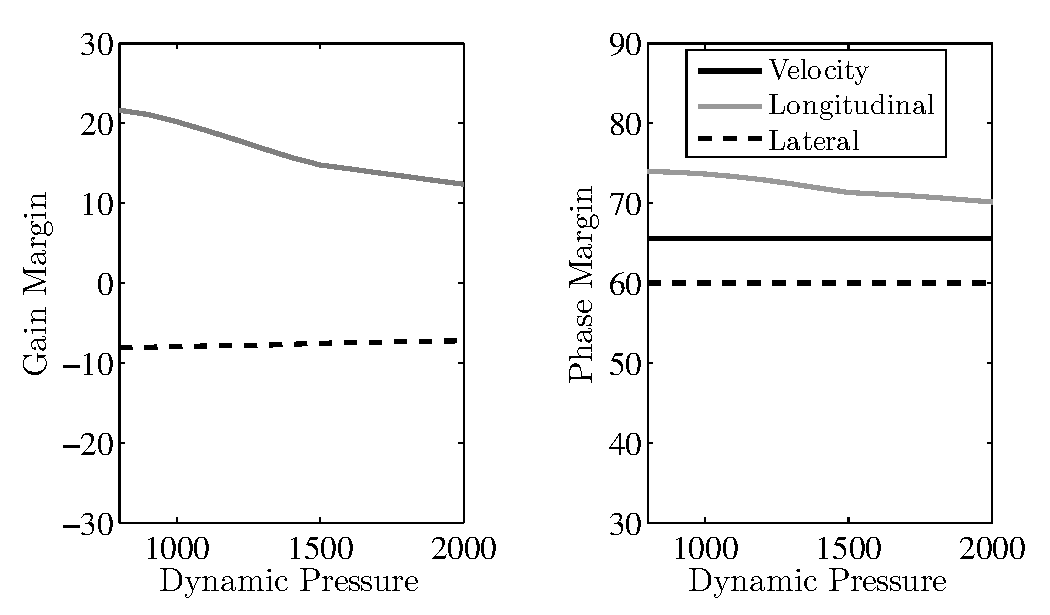
\includegraphics[width=5.0in]{\figurepath/pmgmgainschedule.eps}
    \caption{Gain and phase margin of closed-loop subsystems with gain scheduling \label{fig:pmgmgs}}
  \end{center}
\end{figure}

\begin{figure}[H]
  \begin{center}
    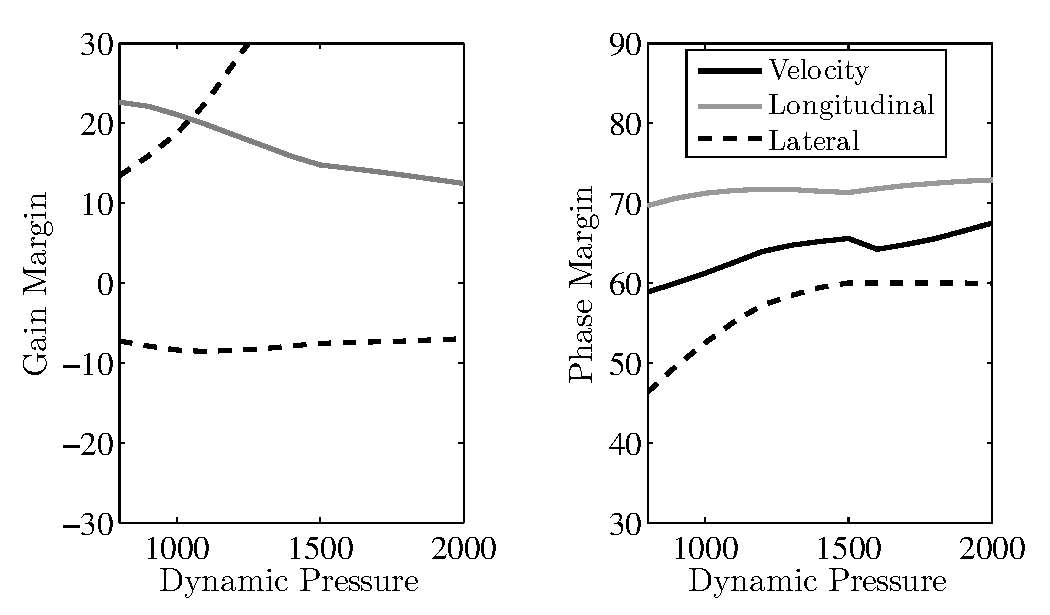
\includegraphics[width=5.0in]{\figurepath/pmgmnogainschedule.eps}
    \caption{Gain and phase margin of closed-loop subsystems without gain scheduling \label{fig:pmgmnogs}}
  \end{center}
\end{figure}

These plots show that the nominal fixed gain that was designed about steady level cruise at Mach 6 maintained satisfactory margins across the entire flight envelope, although there was considerable deterioration in the phase margin at lower dynamic pressures, and gain margin for the lateral-directional subsystem especially.
Across the rest of the dynamic pressure range the gain scheduled controller had margins which were about the same as the nominal fixed gain controller, and even had phase margins which were slightly worse at the higher end of the dynamic pressure range.
It is expected that the increased phase margins of the nominal controller over scheduled controller would come at a cost, and might be at the expense of reduced bandwidth.
However, the method used to determine the feedback gains for this gain-scheduled design were not guaranteed to be the best, and with the full ability to tune the LQR weighting matrices at each point a better design could be achieved through more design iterations.
This method only sought to achieve an overall improvement in the margins over the flight envelope, which it did.

\section{Adaptive Control Design}
\label{sec:adaptivedesign}

The baseline controller in the following section has been designed to have adequate gain and phase margins, and thus should be robust to some reasonable variations in plant parameters and other uncertainties.
However, as uncertainties become excessive, as may often occur in hypersonic vehicles during flight, degradation of the baseline controller will be inevitable, and even a robust baseline controller may not be sufficient to ensure stability.
It is for this reason that an adaptive controller was introduced into the picture.

In the presence of parametric uncertainties, it is unknown how the GHV will respond to input commands during flight.
However, under nominal circumstances the plant is completely known and the baseline controller was designed to achieve an ``ideal'' response to a given input, as determined through the design of the LQR-PI controller.
A model-reference adaptive control (MRAC) structure was chosen as it will attempt to recover this nominal behavior by directly using the error between the ideal, or reference model response and actual, or measured vehicle response to drive parameter adaptation.
This adaptive MRAC controller is designed to ensure good command tracking performance and stability in the presence of these uncertainties\ \cite{book.astrom.1989,slotine.appliednonlinear.1991,narendra.stable.2005}.
In addition, the MRAC control architecture can be added without any modification to the baseline controller.
This baseline-plus-adaptive control architecture is represented by the block diagram shown in Figure~\ref{fig.baseplusadaptiveblock}.
It is noted here that the presence in actuator dynamics as shown in this block diagram cause the commanded control input to differ from the applied control.
This fact is not explicitly taken into account in the control design process, hence the use of $u$ to denote both the commanded control output, and the inputs to the plant.
However, the actuator dynamics were implemented in the evaluation model used for generating various simulation studies.
The control system must be robust enough to tolerate, among other things, the presence of these actuator dynamics.

% TODO@dpwiese - replace this with the actual figure used in SM thesis when submitted
\begin{figure}[h]
  \fontsize{10pt}{10pt}\selectfont
  \begin{center}
    \begin{tikzpicture}[auto, scale=0.85, every node/.style={transform shape}, node distance=1.0cm, >=latex']
      \node[squareblock, minimum height=1cm, minimum width=2cm] (block1){\shortstack[c]{Baseline\\Controller}};
      \node[squareblock, below of=block1, node distance=1.5cm, minimum height=1cm, minimum width=2cm] (block2){\shortstack[c]{Adaptive\\Controller}};
      \matrix[ampersand replacement=\&, row sep=0.5cm, left of=block1,node distance=1cm] (block1in) {%
      \node [coordinate] (b1inA) {};\\
      \node [coordinate] (b1inB) {};\\
      };
      \matrix[ampersand replacement=\&, row sep=0.5cm, left of=block2,node distance=1cm] (block2in) {%
      \node [coordinate] (b2inA) {};\\
      \node [coordinate] (b2inB) {};\\
      };
      \node [left of=b2inB, node distance=0.5cm] (2B) {};
      \node [below of=2B, node distance=0.12cm] (2B2) {};
      \node [left of=b2inA, node distance=1.0cm] (2A) {};
      \node [below of=2A, node distance=0.12cm] (2A2) {};
      \node[whitesum,right of=block1, node distance=2.5cm] (sum1) {};
      \node[squareblock, minimum height=1cm, minimum width=2cm, right of=sum1,node distance=2.5cm] (block3) {Actuators};
      \node[squareblock, minimum height=1cm, minimum width=2cm, right of=block3,node distance=3.0cm] (block4) {Plant};
      \node[squareblock, minimum height=1cm, minimum width=2cm, right of=block4,node distance=4.0cm] (block5) {Sensors};
      \node[output, right of=block5,node distance=2.5cm] (output1) {};
      \node[input, below of=block2,node distance=1.5cm](input2){};
      \draw [->]  (b1inA) + (-2.5cm,0cm) -> node [pos=0.15]{$z_{\text{cmd}}$}  (b1inA);
      \draw [->]  (b1inB) + (-0.5cm,0cm) -> (b1inB);
      \draw [->]  (b2inA) + (-1cm,0cm) -> (b2inA);
      \draw [->]  (b2inB) + (-2.0cm,0cm) -> node[name=TB,node distance=2.5cm]{} (b2inB);
      \draw[->](block5) --  node[name=yi,pos=0.4]{}(output1);
      \draw[-](yi) |- (input2);
      \draw[-](b1inB) + (-0.5cm,0cm) -- (2B2);
      \draw[-](b1inA) + (-1.0cm,0cm) -- (2A2) ;
      \draw[-] (b2inB) + (-2.0cm,0cm) |- (input2);
      \draw[->](block1) -- node[pos=0.22]{$u_{\text{bl}}$} node[pos=0.9]{$+$} (sum1);
      \draw[->](block2) -| node[pos=0.1]{$u_{\text{ad}}$} node[pos=0.9]{$+$} (sum1);
      \draw[->](sum1) -- (block3);
      \draw[->](block3) -- (block4);
      \draw[->](block4) -- (block5);
      \begin{pgfonlayer}{background}
        \path (block1 |- block1)+(-2.5,0.7) node (c) {};
        \path (block2 -| block2)+(3.0,-0.7) node (d) {};
        \path[fill=gray!20, draw, dashed] (c) rectangle (d);
      \end{pgfonlayer}
      \node [below of=block2, node distance = 0.9cm] {Controller};
    \end{tikzpicture}
    \caption{Baseline plus adaptive control block diagram \label{fig.baseplusadaptiveblock}}
  \end{center}
\end{figure}

It was shown in Section~\ref{sec:repofuncertainties} that the nominal plant representation given in Equation (\ref{eqn:plantxp}), when subject to uncertainties, is represented by Equation (\ref{eqn:xdotpunc}) as
\begin{equation}
  \begin{split}
    \dot{x}_{p}&=\bigr(A_{p}+B_{p}\Lambda{W_{p}}^{\top}\bigr)x_{p}+B_{p}\Lambda u \\
    z&=C_{zp}x_{p}
  \end{split}
\end{equation}
This plant model serves as the starting point for the adaptive control design.
In particular, adaptive controllers will be added to the longitudinal and lateral control subsystems, as was shown when introducing the LQR-PI baseline controller in Equation (\ref{lqrpi_linear_ss_eqn}).
Augmenting the uncertain linear plant with an integral error state gives the following
\begin{equation}
  \label{eqn:uncertainss}
  \begin{bmatrix}
    \dot{x}_{p} \\
    \dot{x}_{e}
  \end{bmatrix}=
  \begin{bmatrix}
    A_{p} & 0 \\
    -C_{pz} & 0
  \end{bmatrix}
  \begin{bmatrix}
    x_{p} \\
    x_{e}
  \end{bmatrix}+
  \begin{bmatrix}
    B_{p}\Lambda{W_{p}}^{\top} & 0 \\
    0 & 0
  \end{bmatrix}
  \begin{bmatrix}
    x_{p} \\
    x_{e}
  \end{bmatrix}+
  \begin{bmatrix}
    B_{p} \\
    0
  \end{bmatrix}\Lambda u+
  \begin{bmatrix}
    0 \\
    I
  \end{bmatrix}z_{\text{cmd}}
\end{equation}
Equation (\ref{eqn:uncertainss}) can be expressed using $W^{\top}=[\begin{array}{cc} {W_{p}}^{\top} & 0_{m\times n_{e}} \end{array}]$ as
\begin{equation}
  \begin{bmatrix}
    \dot{x}_{p} \\
    \dot{x}_{e}
  \end{bmatrix}=
  \begin{bmatrix}
    A_{p} & 0 \\
    -C_{pz} & 0
  \end{bmatrix}
  \begin{bmatrix}
    x_{p} \\
    x_{e}
  \end{bmatrix}+
  \begin{bmatrix}
    B_{p} \\
    0
  \end{bmatrix}\Lambda W^{\top}
  \begin{bmatrix}
    x_{p} \\
    x_{e}
  \end{bmatrix}+
  \begin{bmatrix}
    B_{p} \\
    0
  \end{bmatrix}\Lambda u+
  \begin{bmatrix}
    0 \\
    I
  \end{bmatrix}z_{\text{cmd}}
\end{equation}
The integral augmented, uncertain plant for which an adaptive controller will be designed is given by
\begin{equation}
  \label{eqn:uncplant}
  \dot{x}=(A+B\Lambda W^{\top})x+B\Lambda u+B_{\text{ref}}z_{\text{cmd}}
\end{equation}
where $A_{\lambda}=A+B\Lambda W^{\top}$.
This expression reduces to the nominal plant given in Equation (\ref{lqrpiss}) when there is no uncertainty.
The following sections present two model-reference adaptive control strategies.
The first is a classical adaptive controller, and the second is a closed-loop reference model controller.

\subsubsection*{Reference Model}

In order to design a MRAC controller, a suitable reference model is needed.
The reference model defines the desired system performance, with which the plant output is differenced.
It is this difference that is the error signal which drives adaptation.
The classical reference model is given by closing the loop on the nominal plant given by (\ref{eqn:uncplant}) in the absence of uncertainties using the baseline control gain $K_{\text{lqr}}$.
The details concerning the reference model and modifications are provided in the following sections.

\subsection{Classical Model-Reference Adaptive Controller}\label{sec:classicalmrac}

The classical model-reference adaptive controller presented in this section is represented by the block diagram in Figure~\ref{fig:ormblock}.
The approach of adding the adaptive controller on top of the baseline controller is particularly appealing in flight control applications.

\begin{figure}[H]
  \fontsize{10pt}{10pt}\selectfont
  \begin{center}
    \begin{tikzpicture}[auto, scale=1.0, every node/.style={transform shape}, node distance=1.0cm, >=latex']
      \node[squareblock, minimum height=1cm, minimum width=2cm] (block1){\shortstack[c]{Baseline\\Controller}};
      \node[squareblock, below of=block1, node distance=1.5cm, minimum height=1cm, minimum width=2cm] (block2){\shortstack[c]{Adaptive\\Controller}};
      \matrix[ampersand replacement=\&, row sep=0.5cm, left of=block1,node distance=1cm] (block1in) {%
      \node [coordinate] (b1inA) {};\\
      \node [coordinate] (b1inB) {};\\
      };
      \matrix[ampersand replacement=\&, row sep=0.5cm, left of=block2,node distance=1cm] (block2in) {%
      \node [coordinate] (b2inA) {};\\
      \node [coordinate] (b2inB) {};\\
      };
      \node [left of=b2inB, node distance=0.5cm] (2B) {};
      \node [below of=2B, node distance=0.12cm] (2B2) {};
      \node [left of=b2inA, node distance=1.0cm] (2A) {};
      \node [below of=2A, node distance=0.12cm] (2A2) {};
      \node[whitesum,right of=block1, node distance=2.5cm] (sum1) {};
      \node[squareblock, minimum height=1cm, minimum width=2cm, right of=sum1,node distance=2.5cm] (block3) {Plant};
      \node[squareblock, minimum height=1cm, minimum width=2cm, above of=block3,node distance=1.5cm] (block4) {\shortstack[c]{Reference\\Model}};
      \node[whitesum,right of=block3, node distance=2.5cm] (sum2) {};
      \node[output, right of=sum2,node distance=1.5cm] (output1) {};
      \node[input, below of=block2,node distance=1.0cm](input2){};
      \draw [->]  (b1inA) + (-2.5cm,0cm) -> node [pos=0.15]{$z_{\text{cmd}}$}  (b1inA);
      \draw [->]  (b1inB) + (-0.5cm,0cm) -> (b1inB);
      \draw [->]  (b2inA) + (-1cm,0cm) -> (b2inA);
      \draw [->]  (b2inB) + (-0.5cm,0cm) -> node[name=TB,node distance=2.5cm]{} (b2inB);
      \draw[->](block3) -- node[pos=0.5]{$x$} node[pos=0.9]{$+$} node[name=xi,pos=0.4]{} (sum2);
      \draw[->](sum2) --  node[name=yi,pos=0.4]{} node[pos=0.6]{$e^{o}$} (output1);
      \draw[-](xi) |- (input2);
      \draw[-](b1inB) + (-0.5cm,0cm) -- (2B2);
      \draw[-](b1inA) + (-1.0cm,0cm) -- (2A2) ;
      \draw[-] (b2inB) + (-0.5cm,0cm) |- (input2);
      \draw[->](block1) -- node[pos=0.32]{$u_{\text{bl}}$} node[pos=0.9]{$+$} (sum1);
      \draw[->](block2) -| node[pos=0.2]{$u_{\text{ad}}$} node[pos=0.9]{$+$} (sum1);
      \draw[->](sum1) -- node[pos=0.5]{$u$} (block3);
      \draw[->](block4) -| node[pos=0.2]{$x_{m}^{o}$} node[pos=0.9]{$-$} (sum2);
      \draw [->] (b1inA) + (-0.5cm,0cm) |- (block4);
    \end{tikzpicture}
    \caption{Classical model-reference adaptive control architecture\label{fig:ormblock}}
  \end{center}
\end{figure}

The reference model for this classical model-reference adaptive controller is selected by apply the nominal full state feedback controller $u_{\text{bl}}=K_{\text{lqr}}^{\top}x$ to the nominal plant model, where $K_{\text{lqr}}$ is the baseline control gain gain that was calculated to optimize control of the nominal plant.
That is, using the augmented nominal state and input matrices
\begin{equation*}
  A=
  \begin{bmatrix}
    A_{p} & 0 \\
    -C_{pz} & 0
  \end{bmatrix} \quad
  B=
  \begin{bmatrix}
    B_{p} \\
    0
  \end{bmatrix} \quad
  B_{m}=B_{\text{ref}}
\end{equation*}
with the nominal control gain $K_{\text{lqr}}$, the reference model is given by
\begin{equation}
  \label{eqn:xodotm}
  \dot{x}_{m}^{o}=A_{m}x_{m}^{o}+B_{m}z_{\text{cmd}}
\end{equation}
where $A_{m}=A+BK_{\text{lqr}}^{\top}$ is a Hurwitz matrix.
This reference model will provide the nominal response which will be used in calculating the tracking error which will drive adaptation.
With the reference model given in Eq. (\ref{eqn:xodotm}), the tracking error $e^{o}$ is defined as
\begin{equation}
  \label{eqn:eoerror}
  e^{o}=x-x_{m}^{o}
\end{equation}
The adaptive control law is defined as
\begin{equation}
  \label{eqn:uadporm}
  u_{\text{ad}}=\theta^{\top}x
\end{equation}
where $\theta(t) \in \mathbb{R}^{n\times m}$ is the adaptive parameter.
The following adaptive control gain update law is proposed, where $P^{o}=P^{o\top}>0$, and details on the projection operator are found in references\ \cite{lavretskywise.book.2013,PometPraly.1992} and are summarized in Section~\ref{sec:projection}.
\begin{equation}
  \label{eqn:ormupdatelaw}
  \dot{\tilde{\theta}}=\text{Proj}_{\Gamma}\bigr(\theta,-\Gamma^{o} xe^{o\top}P^{o}B\text{sign}(\Lambda)\bigr)
\end{equation}
The total control is given by summing the nominal and adaptive components giving
\begin{equation}
  \label{eqn:utotal}
  \begin{split}
    u&=u_{\text{bl}}+u_{\text{ad}} \\
    &=(K_{\text{lqr}}+\theta)^{\top}x
  \end{split}
\end{equation}
Substituting the control law (\ref{eqn:utotal}) into Equation (\ref{eqn:uncplant}) the closed-loop system becomes
\begin{equation}
  \dot{x}=\left(A+B\Lambda W^{\top}+B\Lambda(\theta+K_{\text{lqr}})^{\top}\right)x+B_{\text{ref}}z_{\text{cmd}}
\end{equation}
Comparing this expression to the reference model, the existence of an ideal feedback gain matrix $\theta^{*}$ that results in perfect reference model tracking can be verified from the following expression.
\begin{equation}
  \label{eqn:matchingcondition}
  A+B\Lambda W^{\top}+B\Lambda(\theta^{*}+K_{\text{lqr}})^{\top}=A+BK_{\text{lqr}}^{\top}
\end{equation}
The adaptive parameter error is defined as
\begin{equation}
  \tilde{\theta}=\theta-\theta^{*}
\end{equation}
Differentiating Equation (\ref{eqn:eoerror}), and substituting (\ref{eqn:uncplant}) and (\ref{eqn:xodotm}) in, the error dynamics can be expressed as
\begin{equation}
  \dot{e}^{o}=A_{\lambda}x+B\Lambda u+B_{\text{ref}}z_{\text{cmd}}-\bigr(A_{m}x_{m}^{o}+B_{m}z_{\text{cmd}}\bigr)
\end{equation}
Substituting Eq. (\ref{eqn:utotal}), and using $B_{m}=B_{\text{ref}}$ the error dynamics become
\begin{equation}
  \dot{e}^{o}=Ax+B\Lambda W^{\top}x+B\Lambda(\theta+K_{\text{lqr}})^{\top}x+B_{\text{ref}}z_{\text{cmd}}-A_{m}x_{m}^{o}-B_{\text{ref}}z_{\text{cmd}}
\end{equation}
Using $A_{m}=A+BK_{\text{lqr}}^{\top}$ and (\ref{eqn:matchingcondition}) the following expression is obtained
\begin{equation}
  A=A_{m}-B\Lambda W^{\top}-B\Lambda(\theta^{*}+K_{\text{lqr}})^{\top}
\end{equation}
This allows the error dynamics to be written as
\begin{equation}
  \dot{e}^{o}=\left(A_{m}-B\Lambda W^{\top}-B\Lambda(\theta^{*}+K_{\text{lqr}})^{\top}+B\Lambda W^{\top}+B\Lambda(\theta+K_{\text{lqr}})^{\top}\right)x-A_{m}x_{m}^{o}
\end{equation}
which finally simplify to
\begin{equation}
  \label{eqn:eodotfin}
  \dot{e}^{o}=A_{m}e^{o}+B\Lambda{\tilde{\theta}}^{\top}x
\end{equation}

The goal of the adaptive controller is to drive the error $e^{o}(t)$ to zero by adjusting the parameter $\theta(t)$.
The following candidate Lyapunov function is proposed, where $\Gamma^{o}\in\mathbb{R}^{n\times n}$ is a symmetric, invertible, positive definite gain matrix, and the operation $|\cdot|$ takes the absolute value of each entry of the matrix argument.

\begin{equation}
  V(e^{o},\tilde{\theta})=e^{o\top}P^{o}e^{o}+\text{tr}\bigr(\tilde{\theta}^{\top}\Gamma^{o-1}\tilde{\theta}|\Lambda|\bigr)
\end{equation}
Differentiating
\begin{equation}
  \label{eqn:Vodot1}
  \dot{V}={\dot{e}}^{o\top}P^{o}e^{o}+e^{o\top}P^{o}\dot{e}^{o}+
  \text{tr}\bigr(\dot{\tilde{\theta}}^{\top}\Gamma^{o-1}\tilde{\theta}|\Lambda|\bigr)
  +\text{tr}\bigr({\tilde{\theta}}^{\top}\Gamma^{o-1}\dot{\tilde{\theta}}|\Lambda|\bigr)
\end{equation}
Substituting Eq. (\ref{eqn:eodotfin}) into Eq. (\ref{eqn:Vodot1}), and letting $-Q^{o}={A_{m}}^{\top}P^{o}+P^{o}A_{m}$ gives
\begin{equation}
  \label{eqn:Vodot2}
  \dot{V}=-e^{o\top}Q^{o}e^{o}+2x^{\top}{\tilde{\theta}}\Lambda{B_{1}}^{\top}P^{o}e^{o}
  +\text{tr}\bigr(\dot{\tilde{\theta}}^{\top}\Gamma^{o-1}\tilde{\theta}|\Lambda|\bigr)
  +\text{tr}\bigr({\tilde{\theta}}^{\top}\Gamma^{o-1}\dot{\tilde{\theta}}|\Lambda|\bigr) \\
\end{equation}
Substituting (\ref{eqn:ormupdatelaw}) into (\ref{eqn:Vodot2}) and letting $y=-xe^{o\top}P^{o}B_{1}\text{sign}(\Lambda)$ gives
\begin{equation}
  \dot{V}=-e^{o\top}Q^{o}e^{o}
  +2\text{tr}\left(\tilde{\theta}^{\top}\bigr(\Gamma^{o-1}\text{Proj}_{\Gamma}(\theta,-\Gamma^{o}y)-y\bigr)|\Lambda|\right)
\end{equation}
The following property of the projection operator as given in Reference\ \cite{lavretskywise.book.2013}
\begin{equation}
  \tilde{\theta}^{\top}\bigr(\Gamma^{-1}\text{Proj}_{\Gamma}(\theta,\Gamma y)-y\bigr)\leq 0
\end{equation}
implies $\dot{V}(e^{o},\theta)\leq 0$.
Thus, the candidate Lyapunov function which was proposed does serve as a valid Lyapunov function for this system.

\subsection{Closed-Loop Model-Reference Adaptive Controller}\label{sec:crmmrac}

In this section, a modification to the classical model-reference adaptive controller described in Section~\ref{sec:classicalmrac} is introduced.
This modification includes an observer-like gain in the reference model, with feedback from the state $x$.
This is referred to as a closed-loop reference model (CRM), and can provide improved transient properties over the classical model-reference adaptive controller, which we denote as the open-loop reference model (ORM) controller\ \cite{gibson.aiaacrm.2012}.
The modified reference model is given by
\begin{equation}
  \label{eqn:xcdotm}
  \dot{x}_{m}^{c}=A_{m}x_{m}^{c}+B_{m}z_{\text{cmd}}-L(x-x_{m}^{c})
\end{equation}
From Equation (\ref{eqn:xcdotm}) it can be seen that the inclusion of the gain $L$ allows the closed-loop reference model response to deviate from that of the open-loop reference model.
In the case when the gain $L$ is reduced to zero, the open-loop reference model is recovered.
This modification to the classical MRAC structure was chosen in an attempt to not only improve the transient response of the system, but also as a potential to provide other improvements such as increased time delay margin, and greater tolerance of parametric uncertainties.

\begin{figure}[h]
  \fontsize{10pt}{10pt}\selectfont
  \begin{center}
    \begin{tikzpicture}[auto, scale=1.0, every node/.style={transform shape}, node distance=1.0cm, >=latex']
      \node[squareblock, minimum height=1cm, minimum width=2cm] (block1){\shortstack[c]{Baseline\\Controller}};
      \node[squareblock, below of=block1, node distance=1.5cm, minimum height=1cm, minimum width=2cm] (block2){\shortstack[c]{Adaptive\\Controller}};
      \matrix[ampersand replacement=\&, row sep=0.5cm, left of=block1,node distance=1cm] (block1in) {%
      \node [coordinate] (b1inA) {};\\
      \node [coordinate] (b1inB) {};\\
      };
      \matrix[ampersand replacement=\&, row sep=0.5cm, left of=block2,node distance=1cm] (block2in) {%
      \node [coordinate] (b2inA) {};\\
      \node [coordinate] (b2inB) {};\\
      };
      \node [left of=b2inB, node distance=0.5cm] (2B) {};
      \node [below of=2B, node distance=0.12cm] (2B2) {};
      \node [left of=b2inA, node distance=1.0cm] (2A) {};
      \node [below of=2A, node distance=0.12cm] (2A2) {};
      \node[whitesum,right of=block1, node distance=2.5cm] (sum1) {};
      \node[squareblock, minimum height=1cm, minimum width=2cm, right of=sum1,node distance=2.5cm] (block3) {Plant};
      \node[squareblock, minimum height=1cm, minimum width=2cm, above of=block3,node distance=1.5cm] (block4) {\shortstack[c]{Reference\\Model}};
      \node [above of=block4, node distance = 1.5cm] (tempnode) {};
      \node[squareblock, minimum height=1cm, minimum width=1cm, right of=tempnode,node distance=1.5cm] (block5) {$L$};
      \node[whitesum,right of=block3, node distance=2.5cm] (sum2) {};
      \node[output, right of=sum2,node distance=2.0cm] (output1) {};
      \node[input, below of=block2,node distance=1.0cm](input2){};
      \draw [->]  (b1inA) + (-2.5cm,0cm) -> node [pos=0.15]{$z_{\text{cmd}}$}  (b1inA);
      \draw [->]  (b1inB) + (-0.5cm,0cm) -> (b1inB);
      \draw [->]  (b2inA) + (-1cm,0cm) -> (b2inA);
      \draw [->]  (b2inB) + (-0.5cm,0cm) -> node[name=TB,node distance=2.5cm]{} (b2inB);
      \draw[->](block3) -- node[pos=0.5]{$x$} node[pos=0.9]{$+$} node[name=xi,pos=0.4]{} (sum2);
      %\draw[->](sum2) --  node[name=yi,pos=0.4]{} node[pos=0.6]{$e^{c}$} (output1);
      \draw[->](sum2) --  node[name=yi,pos=0.4]{} node[pos=0.8]{$e^{c}$} (output1);
      \node [below of=yi, node distance = 0.25cm] (tempnode2) {};
      \draw[-](xi) |- (input2);
      \draw[->](tempnode2) |- (block5);
      \draw[-](b1inB) + (-0.5cm,0cm) -- (2B2);
      \draw[-](b1inA) + (-1.0cm,0cm) -- (2A2) ;
      \draw[-] (b2inB) + (-0.5cm,0cm) |- (input2);
      \draw[->](block1) -- node[pos=0.32]{$u_{\text{bl}}$} node[pos=0.9]{$+$} (sum1);
      \draw[->](block2) -| node[pos=0.2]{$u_{\text{ad}}$} node[pos=0.9]{$+$} (sum1);
      \draw[->](sum1) -- node[pos=0.5]{$u$} (block3);
      \draw[->](block4) -| node[pos=0.2]{$x_{m}^{c}$} node[pos=0.9]{$-$} (sum2);
      \draw [->]  (b1inA) + (-0.5cm,0cm) |- (block4);
      \draw[->](block5) -| (block4);
    \end{tikzpicture}
    \caption{Closed loop reference model adaptive control architecture\label{fig:crmblock}}
  \end{center}
\end{figure}

The modified reference model Jacobian is defined as
\begin{equation}
  \label{eqn:ambar}
  \overline{A}_{m}=A_{m}+L
\end{equation}
and the tracking error is given by
\begin{equation}
  \label{eqn:ecerror}
  e^{c}=x-x_{m}^{c}
\end{equation}
For the CRM adaptive controller, the same adaptive control law as in (\ref{eqn:uadporm}) is used
\begin{equation}
  \label{eqn:uadpcrm}
  u_{\text{ad}}=\theta^{\top}x
\end{equation}
with the following update law
\begin{equation}
  \label{eqn:crmupdatelaw}
  \dot{\tilde{\theta}}=\text{Proj}_{\Gamma}\bigr(\theta,-\Gamma^{c} xe^{c\top}P^{c}B_{1}\text{sign}(\Lambda)\bigr)
\end{equation}
Note that this update law is the same as that in Equation (\ref{eqn:ormupdatelaw}) is used for the ORM adaptive controller, with the exception of the tracking error term $e^{c}$ now being used in the place of $e^{o}$.
The following candidate Lyapunov function is proposed
\begin{equation}
  V(e^{c},\tilde{\theta})=e^{c\top}P^{c}e^{c}+\text{tr}\bigr(\tilde{\theta}^{\top}\Gamma^{-1}\tilde{\theta}|\Lambda|\bigr)
\end{equation}
which has time derivative
\begin{equation}
  \dot{V}=-e^{c\top}Q^{c}e^{c}
  +2\text{tr}\left(\tilde{\theta}^{\top}\bigr(\Gamma^{-1}\text{Proj}_{\Gamma}(\theta,-\Gamma y)-y\bigr)|\Lambda|\right) \\
\end{equation}
As in the ORM case, it can be shown that $\dot{V}(e^{c},\theta)\leq 0$.
Thus, the candidate Lyapunov function which was proposed serves as a valid Lyapunov function for this system.
It can also be shown that $e^{c}\rightarrow e^{o}$ as $t\rightarrow\infty$.

The inclusion of the feedback gain $L$ in the reference model allows the closed-loop reference model response to depart from the open-loop reference model response.
While this can provide improved transient response and other benefits which are observed in simulation, there is also the potential for $L$ to be made sufficiently large so as to deteriorate the time response of the system.
The ideal time response of the system is essentially defined by the open-loop reference model, and the goal is to minimize the tracking error $e^{o}$.
However, in attempting to realize some benefits through the addition of $L$, the closed-loop reference model behavior will be allowed to deviate from the open-loop reference model.
In doing so, while the tracking error $e^{c}$ may be very small, the overall time response of the system may be poor due to large differences between the behavior of the two reference models.
So, while using the error $e^{c}$ to drive adaptation can improve performance, the tracking error $e^{o}$ should still be considered in analyzing performance of the adaptive control system.

\subsection{The Projection Operator}\label{sec:projection}

The projection operator is a means by which the adaptive gain $\theta$ can be bounded.
This is done by specifying a covex function which forms a ball onto which $\dot{\theta}$ is projected.
Consider Figure~\ref{fig:projection}.
The vector $y$ represents $\dot{\theta}$, specified by the update law.
The present value of $\theta$ determines what the projection operator will do, based on where it is in the ball.

\begin{figure}[H]
  \begin{center}
    \psfrag{s}[br][br][1.0]{$\theta^{*}$}
    \psfrag{b}[tc][tc][1.0]{$\theta_{b}$}
    \psfrag{m}[br][br][1.0]{$m=\theta^{*}-\theta_{b}$}
    \psfrag{d}[tc][tc][1.0]{$\nabla f(\theta)$}
    \psfrag{p}[br][br][1.0]{$\text{Proj}(\theta,y)$}
    \psfrag{y}[bc][bc][1.0]{$y$}
    \psfrag{o}[bc][bc][1.0]{$\Omega_{0}$}
    \psfrag{a}[bc][bc][1.0]{$\Omega_{A}$}
    \psfrag{0}[bl][bl][1.0]{$\{\theta|f(\theta)=0\}$}
    \psfrag{1}[bl][bl][1.0]{$\{\theta|f(\theta)=1\}$}
    
\includegraphics[width=3.5in]{\figurepath/projection_v1.eps}
    \caption{The projection operator\label{fig:projection}}
  \end{center}
\end{figure}

The outer radius of the ball is given by $\theta_{\text{max}}$ and determines how large $\|\theta\|$ can get, and the annulus region is defined by $\Delta$.
The projection operator is given by

\begin{equation}
  \text{Proj}_{\Gamma}(\theta,\Gamma y)=
  \begin{cases}
    \Gamma y- \Gamma \frac{(\nabla f(\theta))^{\mathsf{T}}\Gamma y \nabla f(\theta) f(\theta)}{(\nabla f(\theta))^{\mathsf{T}}\Gamma \nabla f(\theta)}, & \text{if }f(\theta)>0\wedge y^{\mathsf{T}}\nabla f(\theta)>0 \\
    \Gamma y, & \text{otherwise}
  \end{cases}
\end{equation}

In order to implement the projection operator in an adaptive law, a convex function is which describes the ball onto which $\dot{\theta}$ will be projected is needed.
Typically the convex functions come in the form of a Euclidean norm squared such as the following.
\begin{equation}
  f(\theta)=\frac{\|\theta\|^{2}-{\theta_{0}}^{2}}{2\Delta{\theta_{0}}+\Delta^{2}}
\end{equation}
where $\theta_{0}$ is the inner radius, defined as $\theta_{0}=\theta_{\text{max}}+\Delta$.
